% Created with jtex v.1.0.15
\documentclass[a4paper,11pt,oneside]{book}
\usepackage[top=2cm, bottom=2cm, left=2cm, right=2cm]{geometry}
\usepackage[T1]{fontenc}
\usepackage[utf8]{inputenc}
\usepackage{lmodern}
\usepackage{hyperref}
\usepackage{graphicx}
\usepackage{caption}
\usepackage{natbib}
\bibliographystyle{abbrvnat}

% Make list items more compact
\usepackage{enumitem}
\setlist[itemize]{noitemsep, topsep=0pt}

%%%%%%%%%%%%%%%%%%%%%%%%%%%%%%%%%%%%%%%%%%%%%%%%%%
%%%%%%%%%%%%%%%%%%%%  imports  %%%%%%%%%%%%%%%%%%%
\usepackage{amsmath}
\usepackage{booktabs}
%%%%%%%%%%%%%%%%%%%%%%%%%%%%%%%%%%%%%%%%%%%%%%%%%%


% Style quotes
\usepackage{xcolor}
% Change links to basic
\hypersetup{
  colorlinks,
  linkcolor={black},
  citecolor={black},
  % urlcolor={blue!80!black}
  urlcolor={black}
}
\usepackage{framed}
\definecolor{quoteshade}{rgb}{0.95,0.95,1}
\renewenvironment{quote}{%
  \def\FrameCommand{%
    \hspace{1pt}%
    {\color{darkblue}\vrule width 2pt}%
    {\color{quoteshade}\vrule width 4pt}%
    \colorbox{quoteshade}%
  }%
  \MakeFramed{\advance\hsize-\width\FrameRestore}
  \noindent\hspace{-8pt}% disable indenting first paragraph
  \begin{adjustwidth}
  \vspace{2pt}\vspace{2pt}%
}
{%
  \vspace{2pt}\end{adjustwidth}\endMakeFramed%
}

\title{\Huge \textbf{A Simple model to study the Complex Cytoplasm}}
\author{\textsc{Mubarrat Mahin Mursalin and Dr. Prof. Stefan Klumpp}}

\begin{document}
\sloppy

\frontmatter
\maketitle

\tableofcontents
% \listoffigures
% \listoftables

\mainmatter

% \include{preface.tex}
% \include{acknowledgements.tex}

\section{Preface}

This work was done for the partial completion of the Master's Degree in the Max Planck School of Matter to Life, at the Universität Göttingen.

\section{Introduction}

\begin{itemize}
\item To be rewritten, Focusing simply on\newline
-Biology is fascinating\newline
-Classical Physics is deterministic\newline
-Biophysics has been trying to put the two together\newline
-The mystery of how matter becomes life
\end{itemize}

The main goal of this paper was to better understand the nature of the inside of a cell. Cells are the basic unit of life and therefor we want to study their complex behavior. Starting from an atomic level description we can build to the cellular level but we lack meaningful methods to quantitatively study systems with such detail. An accurate physical description of the inside of the cell is not only of interest to physicists, but also chemists and biologists, and progress on this topic can lead to innovations in future technologies.

To understand why a studying the inside of a single cell is of importance and interest, we can start with the publications that founded biology. In his works  Charles Darwin describes how multiple species could have come to exist by natural selection. He hypothesized this along his travels across the world, where he was given the opportunity to witness many of these organisms. He noted many physical similarities between different species, different phenotypes. He said these different features served different purposes and they had evolved to do so, because congruent niche existed in the environment where these traits could be useful. A phenotype is beneficial to the organism, if it helps in regards to its survival and reproduction, then it will be persistent in time, and and also said phenotypes are selected for by selection. This idea was controversial, but biological evidence such as homologous structures helped prove Darwin's hypothesis . The question then became, what is the actual mechanism in which the information about these phenotypes are passed on to offspring.

This would only happen later on when DNA was found to be the the code for living systems (that we know of). Before that, the term cell was coined by Leeuwenhoek who developed the first microscopes . After, cells were found to be the basic unit of all living things,and more complex life is just collections of cells. The central dogma of molecular biology has since been the paradigm for thinking in biology on the small scale . The central dogma states that the genome of an organism is defined by its DNAs, then in cell this DNA is read and used as RNAs. RNAs then make proteins. Proteins effect what we see phenotypically, that is to say, protein content controlled by gene expression,leads to the different types of cells we see. The understanding of this is stated as trivial now, but many minds toiled for many years to achieve this level of understanding. Some key discoveries along that pat include works on Nucleic acid concentrations , the structure of DNA , discovery of the ribosome as a machine for making proteins from RNA are just some examples. To limit the discussion to biophysics, yet tie it to general biology, we can say that biology is concerned with the dynamics of living things, which based on their genetic and the external environment.

This is different from physics which is concerned with the motions of objects in time. The most famous early works of physics is Isaac Newton understanding an apple falls, and his laws governing the motion of objects. Since then physics has been concerned with finding equations of motion or dynamics, from the smallest systems to the largest. Specifically quantum mechanics and general relativity have been extremely successful at making predictions in the small and large scales respectively. The works of Albert Einstein that are commonly known are that of the Energy Mass equivalency, $E=mc^2$. However, his lesser known work regarding the photoelectric effect and Brownian motion are what won him the Nobel prize. There are many directions in the study of physics, and often they are not related to each other because of the difference in scales. Biophysics is the study of the motions of living objects in time. It is founded on statistical physics. In the theory section, we will use Einstein's work on Brownian motion as a jumping off point to connect statistical physics and biological systems.

The story would be incomplete without mention of the Chemistry that connects the physical descriptions of matter to the the diversity and beauty in biology. Chemistry is concerned with the properties and behavior of matter.
Just as biology classifies organisms, Chemistry classifies chemicals by their properties. During the 19th century many experiments were done in which new materials were created from naturally occurring matter. These were verified to be pure elements gasses like oxygen and hydrogen and metals like Ytterbium . Properties and interactions of these new elements were tabulated, and trends could be found. These trends are best seen with the periodic table of elements, which places all elements in a table according to similar reactivities and increasing size. Although many of the microscopic details about the elements, such as atomic number or electron configuration were not know until later, detailed descriptions of the nature of the elements, as well as their combinations were known. Chemical reactions allow for the combination and separation (or further convolutions of) different elements. The space of all these combinations is finite, yet so huge that subfield of chemistry exist just to study specific types of combinations. Naturally, biochemistry exists to quench the thirst for knowledge about how living things work based on chemicals. Furthermore, chemistry can neglect many of the microscopic details of the system, and has a language for interactions. These facts make chemistry central in the study of how matter becomes life.

From first glance, it might seem very complicated and futile to study the microscopic structure and dynamics of the inside of a cell. As discussed, the system can be studied from three perspectives, biology chemistry and physics which all seem to provide different views. Physically, the insides of cells are a complex mess of many molecules with many shapes and sizes and compositions. Chemically, a few elements combined in a huge number of ways, react and interact to give rise to the functions we need to survive. Biologically, every part of the system is selected for, and is part of a huge network, both in a cell and an ecosystem. The time scales involved also vary from the shortest fastest quantum dynamics, to the lifetimes of entire organisms.

However, on the contrary, studying the cytoplasm (the inside of a cell), can help answer how ordinary matter becomes life. From a physical perspective, equilibrium statistical mechanics is not sufficient to describe living systems . Biochemical reaction networks exist to describe pathways in a cell, but strives to holistically understand cell functions have been limited. On a biological scale, a quantitative description of whole cells would set a standard for the field. Already today technologies exist which exploit our knowledge of these fields to save lives, lessen suffering, and help on our quest to understand life. Advances like molecular medicine, gene editing, biomedical engineering and synthetic biochemistry are modern examples of how a multi-disciplinary approach to this topic can lead to huge success. In the paper, we will simplify the complex system of a cell into a simple physical model created from biological and chemical data. We hope to show that although many approximations have to be made to study such complex biological systems, quantitative information can still be found to the benefit of physicists, chemists and biologists.

\subsection{Background \& Theory}

\subsubsection{Biology}

\paragraph{Genotype and Phenotypes}

The background of this question starts with identifying cells as a structure in living things. Antonie van Leeuwenhoek, is credited with using his invention of the microscope to study all sorts of samples, some of which were living. He established the field of microscopy by documenting, but also illustrating, what he saw through the lens. This would also set a trend in biology to classify things based on physical observations, also known as phenotypes. Leeuwenhoek also coined the term Cell after his observations of a sample resembled the cells monks reside in. This further goes to show how biology relies on phenotypic descriptions to segregate. Perhaps the most important idea to stem from microscopy is that all living things are made of cells. Although Charles Darwin's work was based on plants and animals, his ideas of evolution of species by natural selection also holds true for cellular life. Furthermore, the components of these living systems are also selected for.

After the establishment of microscopy, scientists studied microscopic systems without the biological classifications nor chemical information we have today. Indeed, this information started from early observations of the nature of microscopic samples. One fact was that some samples were active as compared to others, which were much more inert. This helped convey the idea that microscopic life exists. Another specific observation was a distinction between life made of many cells, and single cellular organisms. Again, that was a very qualitative observation, but we now know that this distinction is actually of Eukaryotic and Prokaryotic cells.

Phenotypically Eukaryotes and Prokaryotes are very different. Not all Eukaryotes are multi cellular, but they all contain internal features that prokaryotes do not. A single cellular organism has to do all the activities associated with life, such as using energy for work consuming food and reproduction only with the machinery it has inside of it. The cells of multi-cellular organisms like you and I, have the luxury of not having to fulfill all these roles by themselves. Multi-cellular organisms can let cells specialize to have specific functions, like muscle cells which help us move or liver cells which help us metabolize. Of course these differences are based on the molecular level, that is to say, these function which the cells can do, are determined by the molecular machines they have.

The distinction between prokaryotic and eukaryotic cells is of specific importance to us in this study. The exact composition of the inside of a cell will vary from cell to cell, even for cells of the same species. Since multi-cellular organisms are also composed of cells, a general rule of thumb is that the difference between cells of different species will be related to how different their genomes are. As described exhaustively in biology,phonemic differences between all living things can be thought of as a (phylogenetic) tree. On the cellular level, the biggest distinction between the insides of cells come from the different domains of life on earth. The three domains bacteria, archaea, and eukaryota arose during the evolution of life, and consequently each domain has features that are adapted for a certain lifestyle. Neglecting arcaea, our discussion will focus on bacteria specifically because eukaryota have membrane bound organelles and are internally inhomogeneous. It should be noted that cells themselves are membrane bound, and we are considering a cytoplasm as the mixture inside this membrane. In eukaryotic cells, the model which we describe later, can also be applied considering only systems enclosed by a membrane and not with multiple separate compartments. The inside of bacteria is homogeneous, except for a central nucleoid which is a DNA rich region. We will start thinking of the cytoplasm of a part of bacteria, inside the membrane but outside the dense nucleoid.

\paragraph{The Central Dogma}

The magic of biology is that the information about the cell, its machines, and indeed the whole organism is written in its genome. Without going over all the discoveries in molecular biology, we will start with the work of Erwin Chargaff. Chargaff's rules says that in a cell the concentrations of the chemicals adenine and thymine are roughly equal, as are the amounts of cytosine and guanine. This was actually of great importance as these chemicals were known to make up DNA, a molecule found in cells, which was observed to related to cell division. Since cell division is one of the steps in reproduction, a key activity of living things, DNA was suspected being the carrier of genetic information. This was described by the works of Watson and Crick , who not only found the physical structure of the DNA molecule, but also probed its role as carrying the information which defines an organism, also known.

Deoxyribose nucleic acids (DNAs) are a double stranded polymer composed of the nucleic acids adenine thymine guanine and cytosine. The central dogma of molecular biology states that DNA is a hard code which defines an organism. That is to say, two organisms are of the same species if they have the same genome. DNA however is not the working memory at the molecular level. That is the role of ribonucleic acids (RNAs), another polymer composed of combinations of the nucleic acids adenine thymine cytosine and uracil. While DNA is physically hard to bend and open, RNA is more flexible, which makes it easier for it to interact with other molecules. In a process called transcription a segment of DNA is copied into RNA, which is analogous to copying information from a larger piece of text to use in a specific instance. These nucleic acid polymers are what compose the genome, or genotype of an organism.

The next step in understanding how the genotype becomes the phenotypes observed in organisms requires knowledge of how activities are done in cells. Although RNA and DNA can carry and move information, more complicated processes such as moving things and using energy require specific chemicals. Proteins are the molecules that do the large variety of work observed in living things. Proteins are also polymers but composed of amino acids, of which there are canonically 20. This allows for a large amount of combinations of amino acids to make a protein, and is what gives rise to the many functionalities of proteins. Proteins have been extensively studied because of their important functions such as applying forces and altering reaction rates. The process in which proteins are made starts with the reading of genetic information (specifically in the form of mRNA) and then converting this to a sequence of amino acids. This process is aptly called transcription, as the genetic information is being transcribed into a functional form.

\subsubsection{Chemistry}

\paragraph{Omics}

We can look at the information space of a living system now from an omics point of view. The genome is based on the DNA of an organism. This DNA can code for many proteins because it be transcript for many RNAs and this layer is called the Transcriptome. At the transcriptome level, the rates of transcription are controlled by transcription factors and this allows for different levels of gene expression. Genes, which is a piece of information defined by a DNA sequence, are expressed as proteins and the collection and abundance of proteins in an organism is called its proteome. Control over the proteins, when they should function, when they should stop, is controlled by post translational modifications and this system we call the epigenome. As the huge number of proteins have a huge number of functions, the leading way of understanding this system has been the metabolic reaction network, also known as the metabolome. One can imagine that a protein may serve a function by affecting some metabolite, for example a molecular motor which does work while consuming adenosine triphosphate ATP. The collection of all these proteins, their metabolites and reaction pathways give rise to all the functions a cell can proform as well as the variety of cellular components. The omics view of the central dogma clearly shows how genetic information on the genomic level can directly lead to the physical structures and functions of living things.

Coincidentally we have just described all the constituents of our model, simply by thinking about the central dogma. We do not consider any molecules related to the genome like DNA, as they would be located in the nucleoid. Instead fragments of DNA and RNA are in the cytoplas as Nucliotides and bases. From the transcriptome we nucleic acids like translational and messenger tRNA and mRNA, as well as proteins which control translation, called translation factors. The last constituent from the transcriptome are large molecular machines, made of both RNA (rRNA) and proteins, called ribosomes. Ribosomes are the location of protein synthesis from the information in mRNA. In bacteria the ribosome is made of multiple subunits (30s \& 50s) which combine to make a full ribosomes (70s and 80s). This brings us to the proteome which mainly contributes proteins which can be classified by their function. We will conisder proteins involved in tRNA synthesis and degredation, transcription, protein folding and degredation and metabolic proteins (enzymes). For a complete picture we consider the metabolome which other than the proteins requires small molecules such as adenosine triphospate. We also consider the fact that ions present in cells at high concentration, and serve many functions such as in controlling protein folding and signaling.

From a chemistry perspective, the metabolome defines a self consistant set of reactions, and thus one can study a cellular process as a chemical reaction. For example, the microscopic details of how a protein does something can be ignored, and can be generalized into macroscopic parameters such as reaction rates. However this gives the illusion that the metabolome can describe all the processes we see in an organism. This is not true because many of the assumptions that work on a part of the reaction network do not apply globally across the network, specifically living systems are active and out of equilibrium. Advances such as the Nobel Prize winning work of Leland H. Hartwell, R. Timothy Hunt, and Paul M. Nurse , showed that general features like the life cycle of cell are conserved between organisms, and selected for. This again shows that although information exists for both the microscopic physical and macroscopic biological level, but a method to directly and precisely connect the two does not yet. Ernest Rutherford is quoted as saying ``All science is either physics or stamp collecting''. This statement doesn't necessarily mean that chemistry and biology are not sufficient nor accurate. Rather it can be seen as the want to describe the amazing phenomena seen in biological systems with the precision and rigor associated with physics.

\paragraph{Soulutions and Mixtures}

\begin{itemize}
\item Solutions and Mixtures \newline
-Some basics (why water solutions)\newline
-Mixing\newline
-Solutions
\end{itemize}

\subsubsection{Physics}

\paragraph{Newton Lagrange and Hamilton}

It is important to remember that all these molecules, DNA RNA proteins are not living, even though they do things to make a system living. As stated before, and in contrast to biology, physics is only concerned with the motions of objects. A single molecule cannot make a system active or out of equilibrium by itself, hence the existence of active matter and collective effects. In fact, any non living object is subject to the deterministic or probabilistic laws of physics. For example Newton's laws of motion say that things do not want to move because of inertia (mass), and accelerate due to forces.

$\vec{F} = m\vec{a}$ with

$\vec{a} = \frac{d\vec{v}}{dt}$ \& $\vec{v} = \frac{d\vec{x}}{dt}$

This means that given the force on an object, its entire movement is known. Lagrangian mechanics extends this idea, by saying what trajectories are actually taken out of many that can be taken.

$L(x, p, t) = T(p, t) - U(x, p, t)$

The only trajectory a system takes is one that minimizes the action.

$S = \int_{t_1}^{t_2} L \, dt$

In Hamiltonian mechanics the time evolution of a system is determined by the Hamiltonian.

$H(\vec{p}, \vec{q}) = \vec{p} \frac{d\vec{q}}{dt} - L = T + U$

Specifically, using the difinition of the Poisson Bracket, where Q is an observable or trajectory

$\{Q_1, Q_2\} = \frac{dQ_1}{d\vec{x}} \frac{dQ_2}{d\vec{p}} - \frac{dQ_1}{d\vec{p}} \frac{dQ_2}{d\vec{x}}$

The quations of motion are known.

$\{\vec{p}, H\} = -\frac{dU}{d\vec{x}} = \frac{d\vec{p}}{dt} = \vec{F}$

$\{\vec{x}, H\} = \frac{d\vec{x}}{dt}$

One can then imagine the trajectory (and all other possible trajectories) of a system in its initial condition. The trajectory as plotted on the coordinates of the Hamiltonian is called the phase space. Although the laws of motion are not yet consistent across length and time scales, the laws of physics are. Quantum mechanics and General relativity are very different. They refer to different processes on different objects, and thus the equations of motion for both theories are wildly different. However key concepts are the same in both theories such as energy minimization and momentum conservation. The main problem we face is that with many body systems is that no analytical solutions exist. Furthermore, with very large systems the calculations become impossible. For this reason we will often refer to statistical properties of the ensamble.

For an observable Q we say that expectation value is

$\langle Q \rangle = \sum_x Q(x)P(x) = \int Q(x)P(x)dx$

We can also define the so called higher moments of a probability distribution as this.

$\mu_{n=1} = \langle x^1 \rangle$

$\langle x^n \rangle = \int_{ -\infty}^{+\infty} (x - c)^n P(x) dx$

In order to study the inside of cells, we will utilize statistical mechanics, and we will show that the key motion is from diffusion.

\paragraph{Diffusion}

A microscopic description of diffusion would come from Robert Brown's work with pollen under the microscope. Meticulously, Brown monitored the positions of individual pollen granules in water. He noticed their sporadic motion, and since then the term for this has been Brownian motion. Today, we posses a larger mathematical vocabulary and know that the trajectories Brown noticed are random walks. As one of the founding works of microscopic motion, further advancements of the details would only come with time.

Adolf Fick studied the diffusion of a colored salt in water. Specifically English chemist Thomas Graham reported the increase of the solution and spread of the colored salt in water, with increases of temperature. Adolf Fick modeled the concept in one dimension, first describing how concentration gradients cause fluxes. Secondly, he considered the time evolution of the concentration due to the fluxes away from high concentration. Consider two boxes next to eachother along the x axis. They each have the same size but different number of particles $\varphi(x, t) = \frac{\#}{V}$. Just from random motion, we expect more particles to move from the box with more particles, and we call this a flux $\vec{J} = \frac{d\#}{dt}$. These ideas are encapsulated in Fick's first,

\begin{equation}
\vec{J} = -D \frac{d\varphi}{dt}
\end{equation}

and second laws.

\begin{equation}
\frac{d\varphi}{dt} = D \frac{d^2\varphi}{dx^2}
\end{equation}

These laws convey the main ideas that any inhomogeneous concentration distributions will relax to a homogeneous one. This process is known as diffusion due to concentration gradients, and Fick's work gave a macroscopic description of it.

The next key works in the path to understanding diffusion came from George Gabriel Stokes. Without going into detail, he developed Stoke's Law

\begin{equation}
\vec{F}_{\text{drag}} = 6\pi\eta r \vec{v}
\end{equation}

which describes the force of drag on a body in water. The specifics of the model he used to derive his law was that of a spherical particle in a laminar flowing Newtonian fluid with a low (zero) Reynold's number. However Stokes did not know of these terms nor details and his law was first an empirical one. Overall this was a key finding in fluid dynamics as it stated how a moving particle is slowed down by a viscous fluid.

This brings us to the work of Albert Einstein that helped earn him his Nobel prize. Einstein wanted a model to describe Brownian motion from microscopic details. Specifically, he believed that the random motion of the suspended particles came from collisions with surrounding particles. Einstein considered how a suspended particle would move in a given time interval in which it collides randomly with surrounding molecules. Mathematically he considered the number density of particles evolving with some timestep tau as a Taylor series expansion.

\begin{equation}
\varphi(x, t + \tau) = \varphi(x, t) + \tau \frac{d\varphi(x, t)}{dt} + \ldots
\end{equation}

This required only the consideration that the particle number is conserved, and is based on the continuity equations. He then showed that this evolution of the number density is equivalent to Fick's laws of diffusion. He then described the fundamental solution to the diffusion equation as having the form

\begin{equation}
\varphi(x, t) = \frac{N}{\sqrt{4\pi D t}} e^{-\frac{x^2}{4Dt}}
\end{equation}

with

$\langle x \rangle=0$ \& $\langle x^2 \rangle = 2Dt$

More importantly, Einstein was able to define the coefficient from Fick's equation in terms of mean squared displacement of the particle. Then he related this coefficent again to measurable physical quantities like the temperature.

Almost simultaneously, Marian Smoluchowski developed another explanation of the observations of Brownian motion. Combining the Einsteins previous work on the Kinetic theory of molecules, he concluded that diffusion coefficient from Fick's law is determined by the temperature

\begin{equation}
D = \mu k_b T = \frac{k_b T}{6\pi\eta r}
\end{equation}

and the mobility of the particle.

\begin{equation}
\mu = \frac{1}{6\pi\eta r}
\end{equation}

Combining the works of Stokes's Einstein and Smoluchowski, we arrive at a key relation.

\begin{equation}
\frac{\langle x^2 \rangle}{t} = \frac{K_b T}{6\pi\eta r}
\end{equation}

We now have intuition about the diffusion coefficient, which is dependent on the size of the molecule the viscosity of the surrounding fluid and the temperature of the system. Further more, we know from the fundamental solution the the diffusion equation, that on average the particle does not move
but the mean squared displacement of the particle
increases linearly with time. The implications of these works are actually still understated. They not only described the motions of microscopic objects, but also proved further the existence of atoms.

\paragraph{Langevin Equation}

One more key milestone in the study of diffusion and statistical mechanics was the development of the Langevin equation of motion. Paul Langevin wanted a macroscopic description of the motion of a particle with some random driving force. This was analogous to a macroscopic description of diffusion as the motion of a diffusing particle is caused by random collisions with microscopic particles from its surroundings.

To quantify this random force Langevin considered that the noise should obey two properties, on average the force is random and thus zero,

\begin{equation}
\langle n(t) \rangle = 0
\end{equation}

and has no particle particle nor time correlations due to the delta functions.

\begin{equation}
\langle \vec{n}_1(t_1) \vec{n}_2(t_2) \rangle = \delta_{12} \delta(t_1 - t_2)
\end{equation}

Considering only a non-interacting particle surrounded by a microscopic fluid he wrote the equation of motion in the form

$\vec{F} = m \frac{d\vec{v}}{dt} = \vec{n}(t)$

With this he was able to show the distribution of velocities was fixed

$\langle x \rangle = 0 \, \text{and} \, \langle v \rangle = C$

However with only a random noise term the second moment of the distribution increases with time

$\langle v^2 \rangle \propto t$

However if a drag term is introduced in the exact form

\begin{equation}
m\frac{dv}{dt} = -\gamma v(t) + n(t)
\end{equation}

then the mean position of the particle is zero and mean squared displacement is related to the strength of the noise, which is the Stokes-Einstein relation.

$\gamma = 6\pi\eta r$

The drag force can also be derived as a random force but is also velocity dependent as more collisions will occur in the direction of travel. The implications of this is quite profound. It says that due to temperature, nature will give you a random force which pushes you, but one cant take advantage of it because the same random process will also hinder you. The Stokes-Einstein relation is only one example of this, and the generalized idea is called a fluctuation dissipation theorem. With the Langevin equation of motion, we now have a method to drive particles which we want to diffuse. This innovation was huge in the field of statistical mechanics, as we developed a stochastic differential equation of motion.

\begin{itemize}
\item Possible things to add \newline
-Fokker Planck \newline
-Fastest possible reactions as inspiration (Smoluchouski)
\end{itemize}

\paragraph{The Liquid State}

Caught up in our discussion of the motion of the molecules we neglected the fluid these objects exist in. In equation ...

\begin{itemize}
\item Complex Mixtures \newline
-Reaction Diffusion \newline
-LLPS \newline
-Glasses
\end{itemize}

\paragraph{Theory from our work}

\begin{itemize}
\item Theory specific to this work \newline
-The cytoplasm as spheres \newline
-Our interaction model \newline
-Measures used in analysis
\end{itemize}

\section{Methods}

\begin{itemize}
\item This Section is to be updated
\end{itemize}

\subsection{Making Soup; Building a cytoplasm}

We started from the work of Feig et al as a complete annotated database of the contents of a piece of cytoplasm. This paper had a database which contained many constituents with concentrations. It was supplemented with data from PaxDB and UniProt DB which are proteomics and genomics databases respectively. This was done to account for proteins in the Feig et al data which were in PDB format. Our final database has 452 constituents with some species having a minimum concentration of 1um. From this database we can generalize our average cytoplasm to be in a box of (100nm)\^3 with 94.81\% filled with water molecules.

From the model cytoplasm we also created a test system. Our aim was to
create an analogous system to the full cytoplasm, which means keeping physical qualities such as mass and radii abundance, while simplifying the system. The main quantities of the cytoplasm constituents were charge and radius so the test system was modeled using 9 molecule types corresponding to 3 radii small medium and large and 3 types of charges positive negative and neutral. The abundances of the constituents were made to represent volume fractions in the real cytoplasm.

\begin{table}
\centering
\caption[]{Information about our studied systems}
\label{table}
\begin{tabular}{p{\dimexpr 0.167\linewidth-2\tabcolsep}p{\dimexpr 0.167\linewidth-2\tabcolsep}p{\dimexpr 0.167\linewidth-2\tabcolsep}p{\dimexpr 0.167\linewidth-2\tabcolsep}p{\dimexpr 0.167\linewidth-2\tabcolsep}p{\dimexpr 0.167\linewidth-2\tabcolsep}}
\toprule
System Name & Num. of Molecules & Num. of Molecular Species & Net Charge & Specific interactions & Description \\
\hline
IntCytoSys & 42,809 & 445 & -12,710 & Yes & Full model cytoplasm with specific interactions \\
CytoSys & 42,809 & 445 & -12,710 & No & Full model cytoplasm \\
SymTestSys & 4,287 & 3 & 0 & No & Reduced size test system with no net charge \\
NoQSymTestSys & 4,287 & 3 & 0 & No & Reduced size test system with no net charge nor charge effects \\
TestSys & 4,278 & 3 & -2,039 & No & Reduced size system, proportional to model \\
\bottomrule
\end{tabular}
\end{table}

\subsection{The Simulation Engine}

Data from our database was given as an input to a simulation engine built on the HOOMD-Blue library on Python. HOOMD-Blue was selected for its ease of use, good documentation, and for its ability to run molecular dynamics simulations of GPUs.

The simulation box was constructed according to occupied volume fraction. The total volume of the box was set so that the molecules from database would occupy a specified volume fraction. To create the system, a scaled up box was filled up with molecules in the database. These molecules were placed randomly with the PACMOL software implemented in python via the Mbuild library.

Multiple steps were taken to ensure that while each instance of the simulation was different with the same constituents, each instance was also thoroughly equilibrated before any quantities of interest were recorded. Specifically, the enlarged box filled with molecules was shrunk to the correct size. After compression, the system was allowed to equilibrate with potentials that were both cut off at a small radius, and modified to raise the potential energy minimum. This was rationalized as erroneous results would only result if there was significant overlap of the spheres representing the molecules, and this would not happen from the cutoff nor the boosted potential. The pressure and potential energy was monitored during the equilibration to verify that the system had stabilized.

Molecular dynamics simulations of this equilibrated system was run as the main computer experiment in this study. The specific data that was given to the simulation was a simulation box filled with molecules, an n-n pairwise interaction matrix with n as the number of species which scales the LJ epsilon parameter, physical parameters of temperature viscosity and ionic strength, and simulation constraints such as the timestep the total time and how often to write data to the trajectory. Very specifically, at each timestep the simulation box was initialized. For each particle the force was calculated as generated from pairwise LJ and Yukawa interactions with every other particle in the cutoff radius. During said timestep, the force and a random noise term drove the particles, while a viscous dampening slowed them as according to brownian dynamics. The usual simulation was done with in a box of size (100nm)\^3, with a timestep of 0.1 femtoseconds, at 30C and 150mM ionic strength and a viscosity of 1 (water). HOOMD-Blue wrote the trajectory at a given rate as a binary gsd file. To minimize file sizes, the simulation was broken into 2 time regimes, slow and fast. 2 trajectories were created from 1 simulation, with 2 write rates, with the slow writer ending after a certain number of steps. The data was stitched together from both trajectories during analysis.

To monitor the accuracy of the simulation, the kinetic, potential and total energies along with the kinetic temperature and pressure were monitored. This was done by extracting these quantities along with others at each trajectory step. Stability was determined when the total energy, potential energy and pressure stabilized during equilibration.

To monitor the mean squared displacement of the particles from the trajectory, the Freud library was used. The library is able to calculate the MSD for each particle in the trajectory over a sliding time window, which decreases computational cost. For a certain species the MSD was averaged over all particles of said species. Other quantities derived from the MSD v time such as log MSD v log time was also calculated from the averaged MSDs.

\section{Results}

\subsection{Constituents of the cytoplasm}

\begin{figure}[!htbp]
\centering
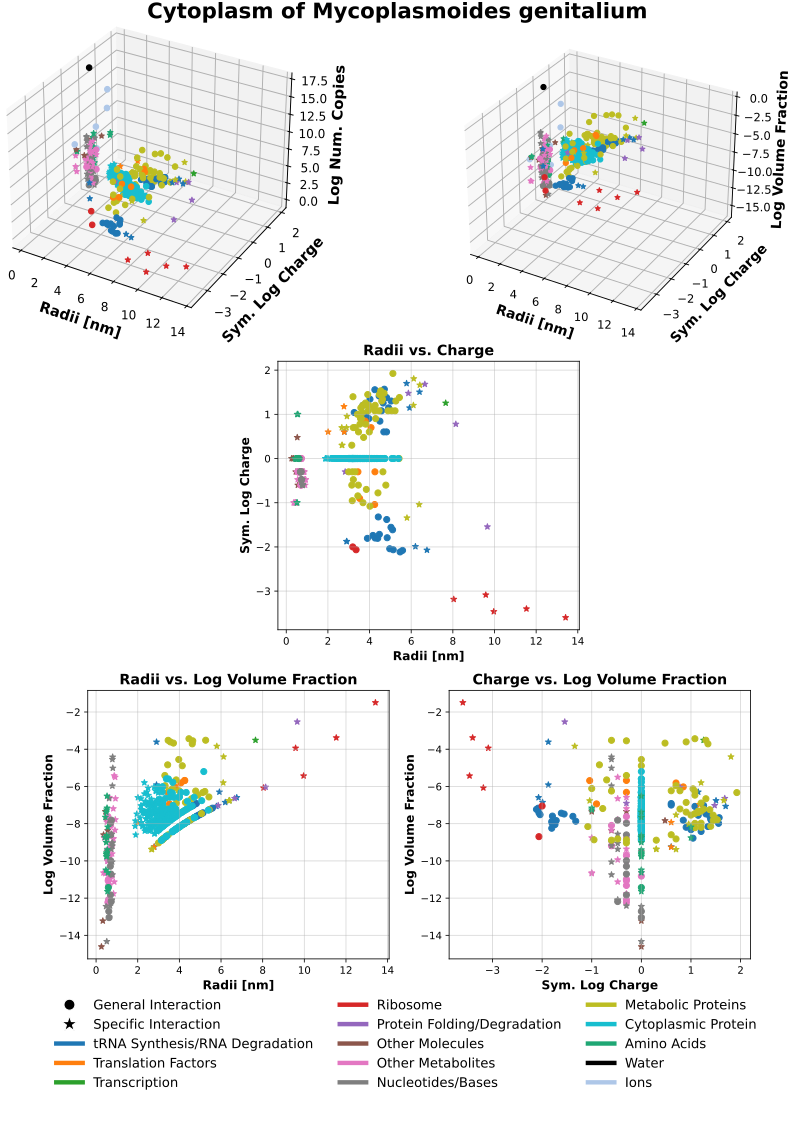
\includegraphics[width=0.7\linewidth]{files/Fig1-77a0883bc22d4aa609016ce8a1ec042f.png}
\caption[]{Plots showing the molecular constiuents of Mycoplasma Genitalium, based on size charge and abundance.}
\label{Fig1_OmicsPlot}
\end{figure}

\begin{itemize}
\item Results from Modelling the Cytoplasm\begin{itemize}
\item Mostly Water
\item Ions are a huge portion
\item Some clear grouping of constituents
\item Skew towards negative charge
\item Ribosomes are few but very big
\end{itemize}
\end{itemize}

\subsection{Possible Interactions of the model}

\begin{figure}[!htbp]
\centering
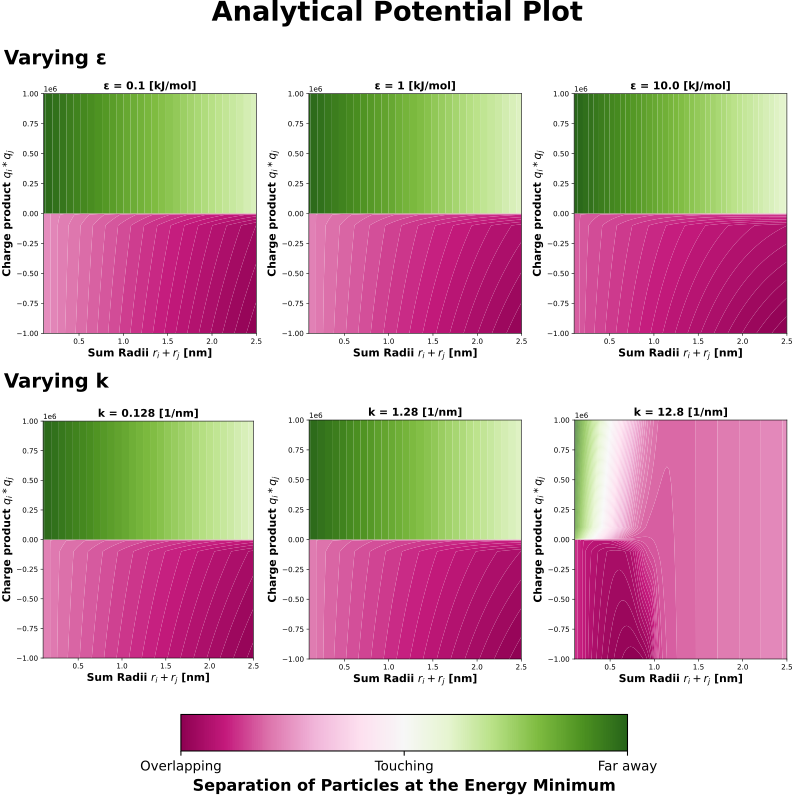
\includegraphics[width=0.7\linewidth]{files/Fig2-4a634fb40ba25fe916b6010c8907b16e.png}
\caption[]{Analytical Plots showing all possible effects of the potential, on molecules of diffrent size and charge.}
\label{Fig2_PotentialPlot}
\end{figure}

\begin{itemize}
\item Analytical Results\begin{itemize}
\item Our model allows both overlapping and diffuse phase of particles
\end{itemize}
\end{itemize}

\subsection{Equilibration}

\begin{itemize}
\item Equilibrium Results\begin{itemize}
\item We never reach true equilibrium
\item Sampling many time ranges, we find that energies and pressure stabilize
\item Pressure drops but stabilizes, like rarified gas
\end{itemize}
\end{itemize}

\begin{figure}[!htbp]
\centering
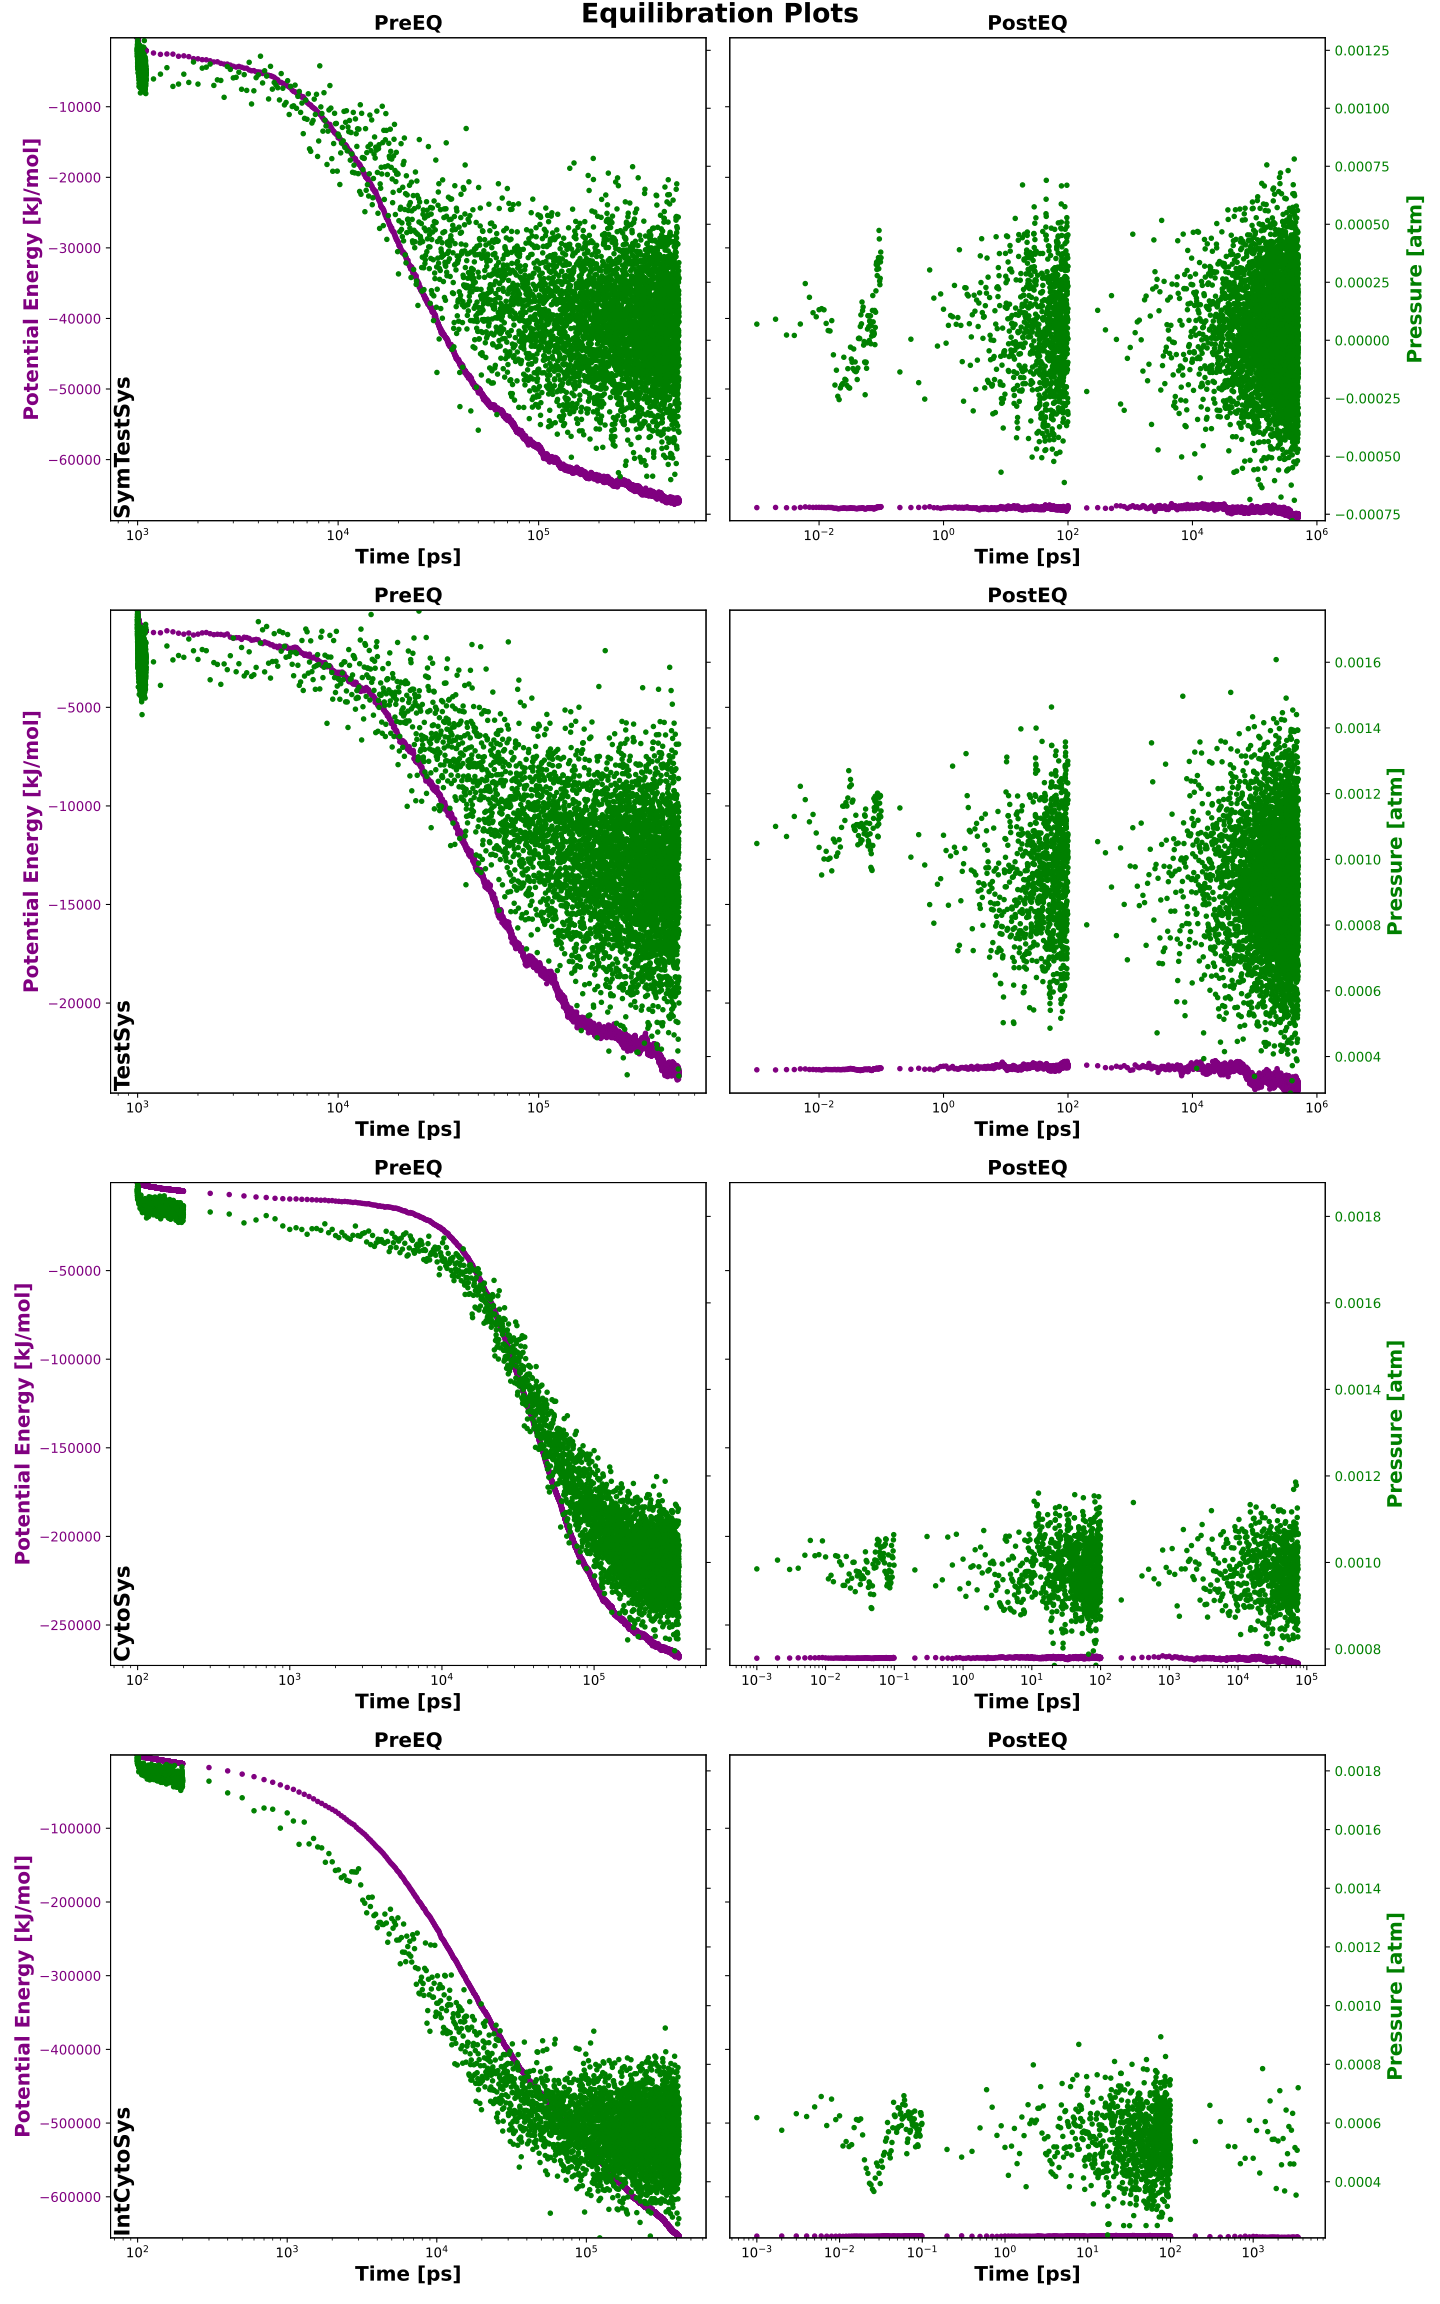
\includegraphics[width=0.7\linewidth]{files/Fig3-c8f52112ab9c36b95917d32f74d7df9b.png}
\caption[]{Plots showing the Pressure and Potential energies of various systems as calculated with the Freud library. The data was used to determine when the simulation data (MSD,Cluster statistics, etc) could be calculated without worry of equilibration.}
\label{Fig3_EQ}
\end{figure}

\subsection{Simulation Data}

\begin{itemize}
\item Simulation Results\begin{itemize}
\item Net charge determines diffuse phase
\item MSD is not linear with time
\item MSD also no glassy
\item Reproducing anomalous diffusion on experimental time scales
\item Clusters are log-normal distributed\begin{itemize}
\item Mean zero, skew
\end{itemize}


\item RDF's show some known structures
\item RDFs also inconclusive
\end{itemize}
\end{itemize}

\begin{figure}[!htbp]
\centering
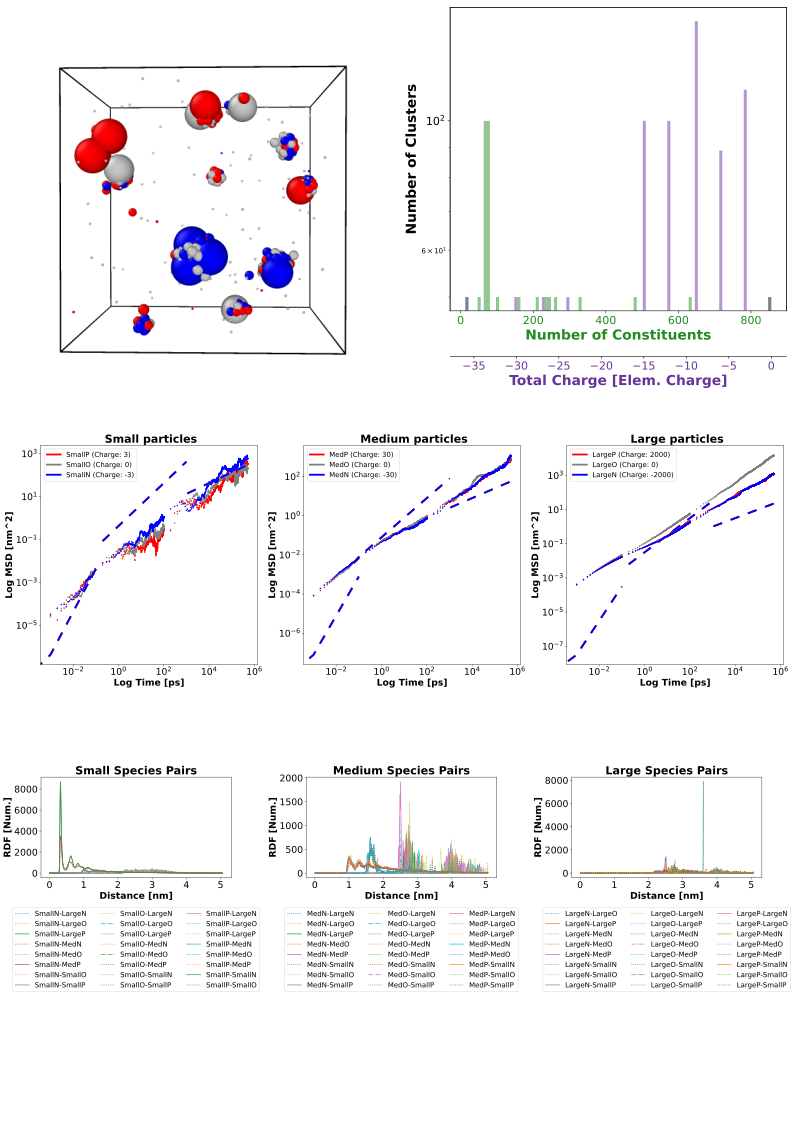
\includegraphics[width=0.7\linewidth]{files/Fig4-58e6dad7889c9d6eaaa4abc74e3534eb.png}
\caption[]{Simulation data from the Symmetric Test System. The dashed lines in the MSD Plots are to guide the eye to the left $\propto t^2$ middle $\propto t$ and right $\propto t^{1/2}$ behaviours.}
\label{Fig4_SymTestSys}
\end{figure}

\begin{figure}[!htbp]
\centering
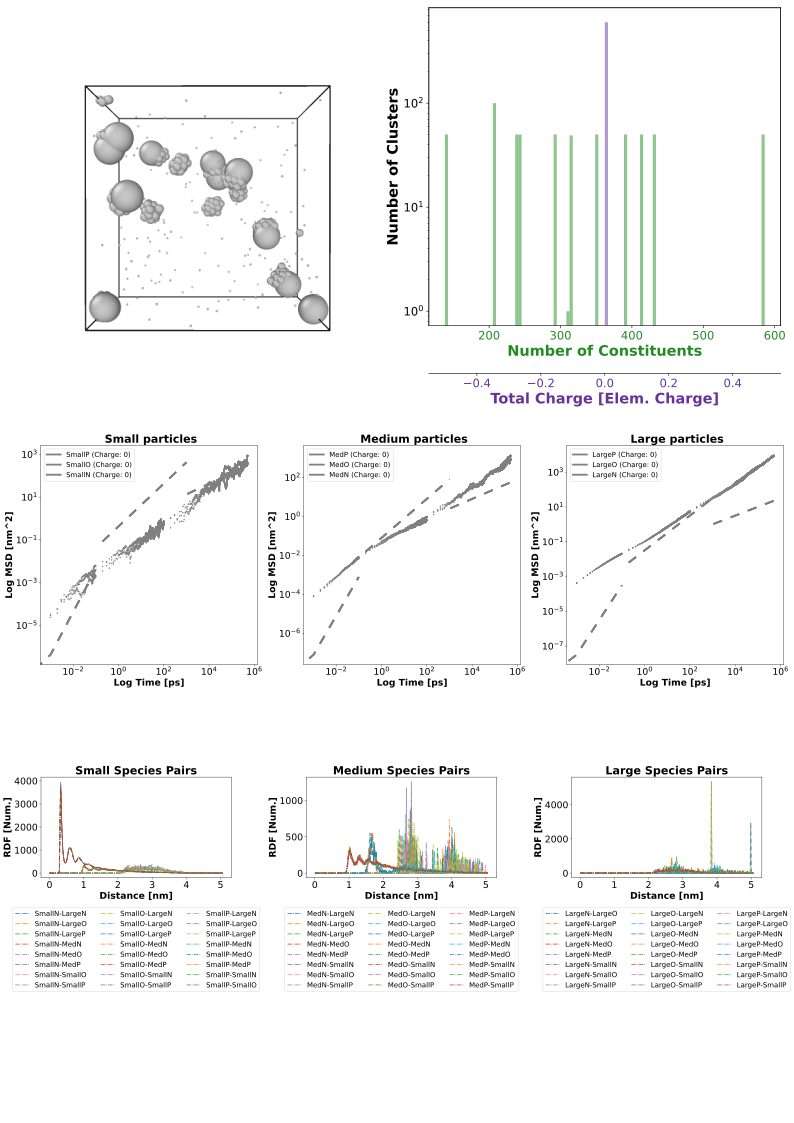
\includegraphics[width=0.7\linewidth]{files/Fig5-85672235d6e59a344ebdc8dfebe8a845.png}
\caption[]{Simulation data from the Symmetric Test System with no charge. The dashed lines in the MSD Plots are to guide the eye to the left $\propto t^2$ middle $\propto t$ and right $\propto t^{1/2}$ behaviours.}
\label{Fig5_NoQSymTestSys}
\end{figure}

\begin{figure}[!htbp]
\centering
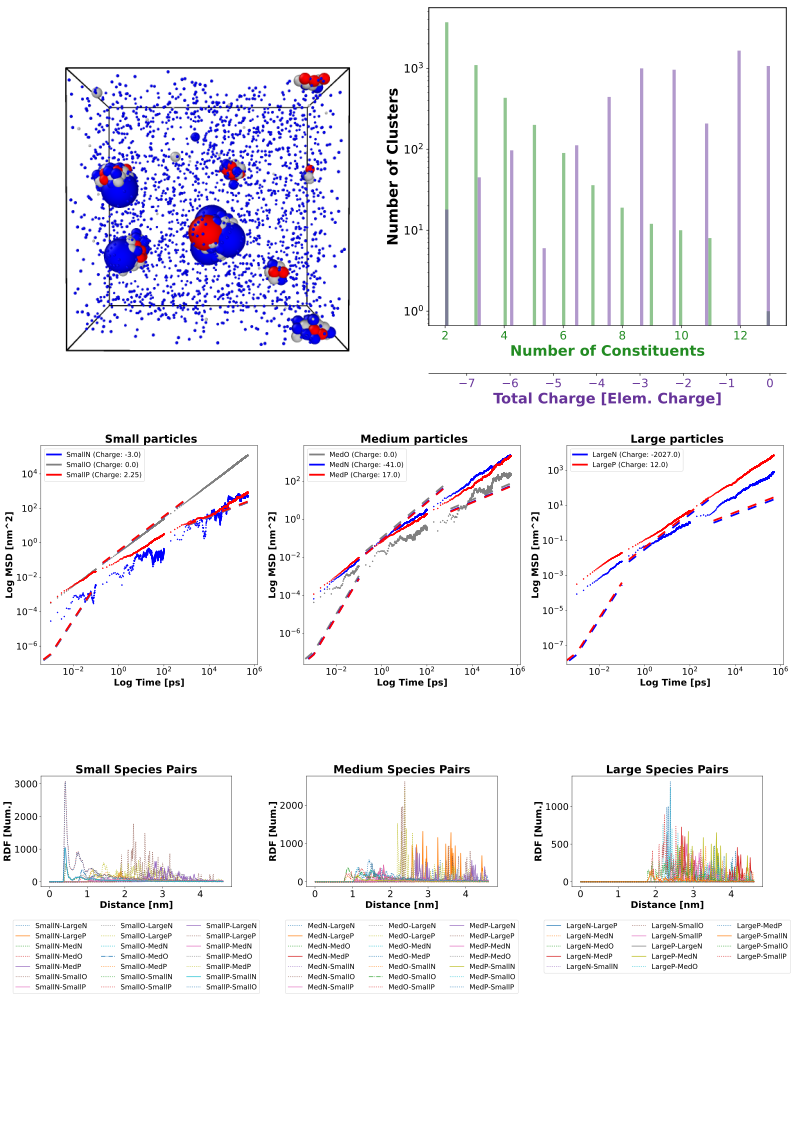
\includegraphics[width=0.7\linewidth]{files/Fig6-a7ed5a88b4f52cd6f742db9bb56d35f3.png}
\caption[]{Simulation data from the minimal Test System. The dashed lines in the MSD Plots are to guide the eye to the left $\propto t^2$ middle $\propto t$ and right $\propto t^{1/2}$ behaviours.}
\label{Fig6_TestSys}
\end{figure}

\begin{figure}[!htbp]
\centering
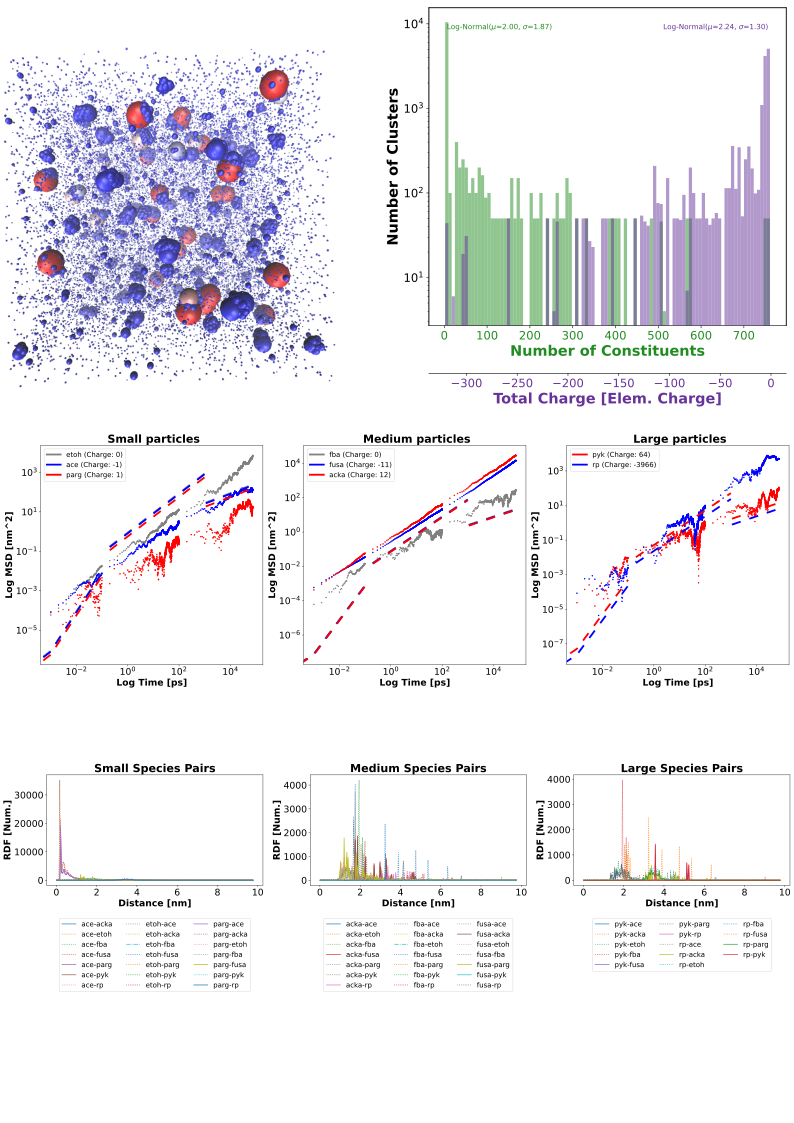
\includegraphics[width=0.7\linewidth]{files/Fig7-52255c465b726bd0729aff0b90c8f0ed.png}
\caption[]{Simulation data from the full cytoplasm, except with no specific interactions. The dashed lines in the MSD Plots are to guide the eye to the left $\propto t^2$ middle $\propto t$ and right $\propto t^{1/2}$ behaviours.}
\label{Fig7_NoQTestSys}
\end{figure}

\begin{figure}[!htbp]
\centering
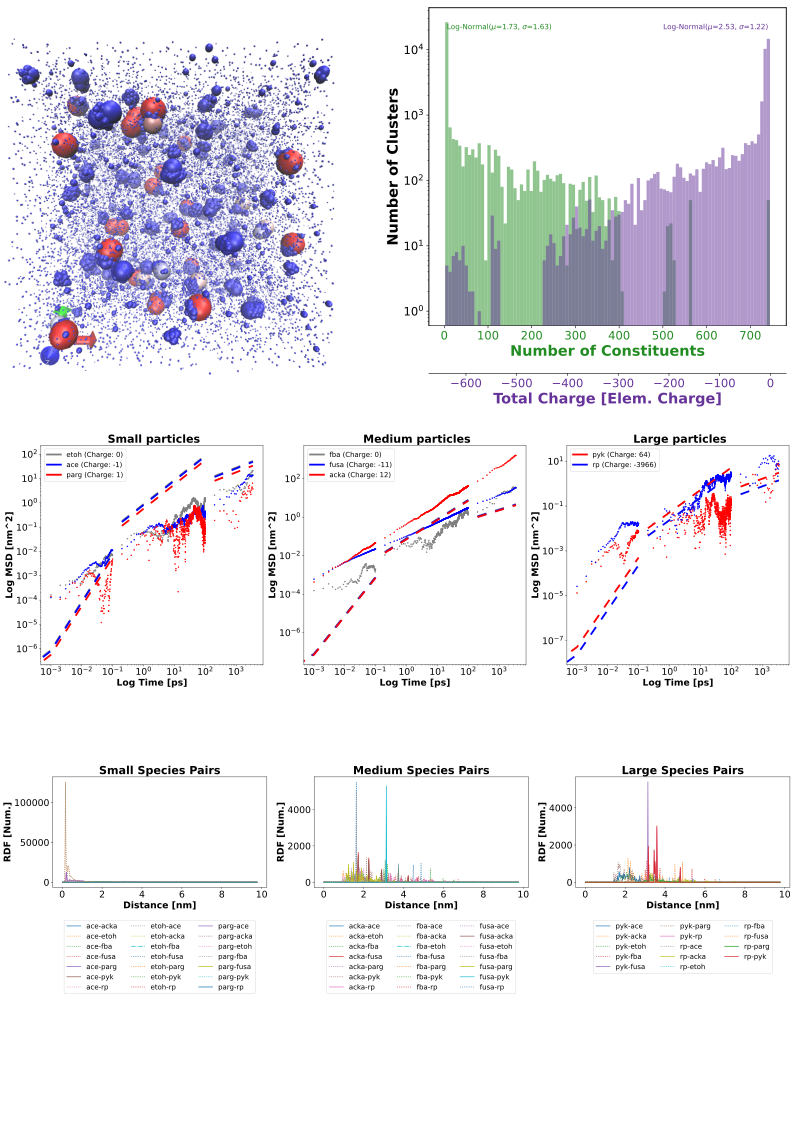
\includegraphics[width=0.7\linewidth]{files/Fig8-efc86aafad27c0dca716926433b3ab15.png}
\caption[]{Simulation data from the full cytoplasm, with specific interactions. The dashed lines in the MSD Plots are to guide the eye to the left $\propto t^2$ middle $\propto t$ and right $\propto t^{1/2}$ behaviours.}
\label{Fig8_CytoSys}
\end{figure}

\subsection{Parameter Scans}

\begin{itemize}
\item Parameter Scan Results\begin{itemize}
\item Strong interactions and low screening means fast cluster formation
\item Global rate controlled by global parameters of epsilon and kappa
\end{itemize}
\end{itemize}

\begin{figure}[!htbp]
\centering
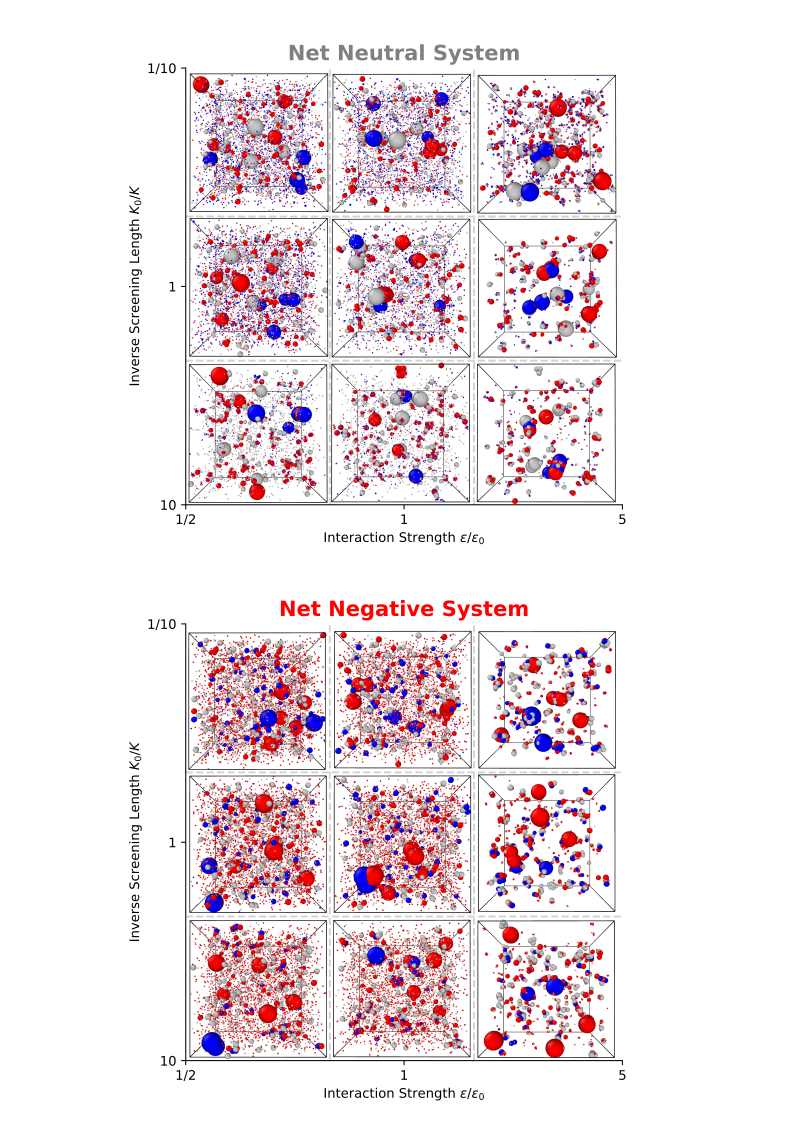
\includegraphics[width=0.7\linewidth]{files/Fig9-b4858396f6517661b798f42ca198a015.png}
\caption[]{Qualitative graph showing the test systems simulated for a variety of parameters. All the simulations were run for the same amount of time.}
\label{Fig9ParamScan}
\end{figure}

\section{Discussion \& Conclusions}

\begin{itemize}
\item The model is okay, need better tools and theory to study chaotic statistical systems\newline
-Pros and Cons of the model\newline
-The Limiting case of explicit water and ions\newline
-HPMC as an alternative simulation


\item Living cells need active control over the cytoplasm\newline
-Cytoplasm is non ergodic\newline
-Cell must have control to avoid equilibrium\newline
-EQ is often death or disease, examples\newline
-Relation between controlled dynamics and controlled glassy state
\end{itemize}



\end{document}
